\documentclass[UTF8,fontset=none,12pt]{ctexart}

\setCJKmainfont{Songti SC}
\setCJKsansfont{PingFang SC}
\setCJKmonofont{Songti SC}

\usepackage[a4paper,margin=2.35cm]{geometry}
\usepackage{amsmath,amssymb,amsthm,mathtools,bm}
\usepackage{graphicx}
\usepackage{float}
\usepackage{booktabs}
\usepackage{enumitem}
\usepackage[hidelinks]{hyperref}

\newcommand{\C}{\mathbb{C}}
\newcommand{\R}{\mathbb{R}}
\newcommand{\range}{\operatorname{range}}
\newcommand{\nullspace}{\operatorname{null}}
\newcommand{\rank}{\operatorname{rank}}
\newcommand{\Span}{\operatorname{span}}
\theoremstyle{definition}
\newtheorem{theorem}{定理}
\renewcommand{\thetheorem}{7.\arabic{theorem}}

\title{数值线性代数\quad 第 7 讲：QR 分解}
\author{Lloyd N. Trefethen、David Bau III\quad 中文阅读版}
\date{}

\begin{document}
\maketitle
\pagestyle{plain}

上一讲介绍了投影算子.本讲转向一种构造正交基的基本算法：QR 分解.它把一个矩阵写成正交（或酉）矩阵与上三角矩阵的乘积，是正交化、最小二乘和许多数值算法的共同入口.

\section*{QR 分解}

设 $A=[a_1\ \cdots\ a_n]\in\C^{m\times n}$，且 $m\ge n$.如果 $A$ 满列秩，则它的列向量依次生成一串嵌套子空间：
\[
    \langle a_1\rangle\subseteq\langle a_1,a_2\rangle\subseteq\langle a_1,a_2,a_3\rangle\subseteq\cdots.
\]
我们的目标是构造单位向量 $q_1,\ldots,q_n$，使得对 $j=1,\ldots,n$，都有
\begin{equation}
    \langle q_1,\ldots,q_j\rangle=\langle a_1,\ldots,a_j\rangle.
    \tag{7.1}
\end{equation}
如果这些向量还彼此正交，那么每个 $a_j$ 都可以在前 $j$ 个 $q_i$ 的基础上展开.于是有
\begin{equation}
    A=[a_1\ \cdots\ a_n]
    =[q_1\ \cdots\ q_n]
    \begin{bmatrix}
        r_{11}&r_{12}&\cdots&r_{1n}\\
        0&r_{22}&\cdots&r_{2n}\\
        \vdots&\ddots&\ddots&\vdots\\
        0&\cdots&0&r_{nn}
    \end{bmatrix}
    =\widehat Q\widehat R.
    \tag{7.2}
\end{equation}
其中 $\widehat Q=[q_1\ \cdots\ q_n]$ 是列标准正交的 $m\times n$ 矩阵，$\widehat R$ 是 $n\times n$ 上三角矩阵.对每一列逐项写开，就是
\begin{equation}
\begin{aligned}
    a_1&=r_{11}q_1,\\
    a_2&=r_{12}q_1+r_{22}q_2,\\
    a_3&=r_{13}q_1+r_{23}q_2+r_{33}q_3,\\
    &\ \vdots\\[-0.5em]
    a_n&=r_{1n}q_1+r_{2n}q_2+\cdots+r_{nn}q_n.
\end{aligned}
\tag{7.3}
\end{equation}
式 (7.2) 称为 $A$ 的\textbf{约化 QR 分解}.在满列秩情形中，所有对角元 $r_{kk}$ 都非零.

还可以把 $\widehat Q$ 补成一个 $m\times m$ 的酉矩阵 $Q$，并在 $\widehat R$ 的底部补上 $m-n$ 行零，从而得到一个 $m\times n$ 的上三角矩阵 $R$.这给出完整 QR 分解
\begin{equation}
    A=QR.
    \tag{7.4}
\end{equation}
完整分解中，$Q$ 的后 $m-n$ 列乘上 $R$ 中对应的零行，因此它们不会改变乘积.当 $A$ 满列秩时，这些列构成 $\range(A)^\perp=\nullspace(A^*)$ 的一组标准正交基.

\begin{figure}[H]
    \centering
    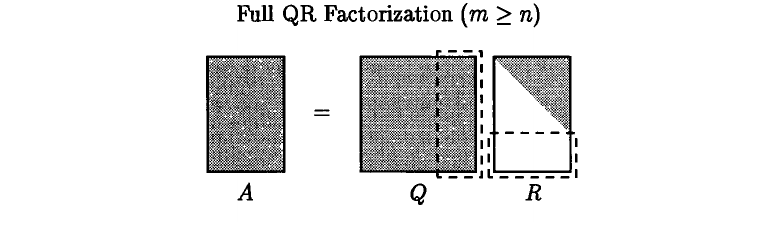
\includegraphics[width=0.72\linewidth]{../assets/figure-7-full-qr.png}
    \caption{完整 QR 分解的结构图（$m\ge n$）.虚线部分表示为了从约化分解扩展到完整分解而补入的列和零行.}
    \label{fig:full-qr}
\end{figure}

在约化 QR 分解中，删去完整分解中不参与乘积的列和行，得到 $\widehat Q\in\C^{m\times n}$、$\widehat R\in\C^{n\times n}$. $\widehat R$ 的行不必包含零行.

\begin{figure}[H]
    \centering
    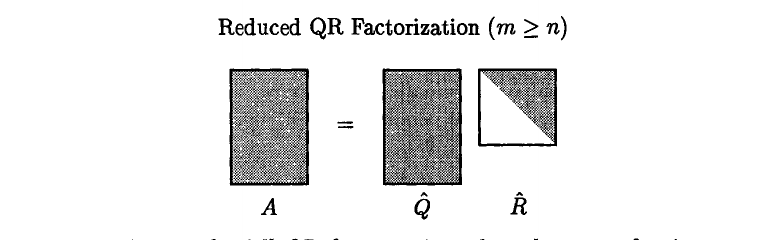
\includegraphics[width=0.72\linewidth]{../assets/figure-7-reduced-qr.png}
    \caption{约化 QR 分解的结构图（$m\ge n$）.}
    \label{fig:reduced-qr}
\end{figure}

\section*{Gram--Schmidt 正交化}

第 $j$ 步需要在 $\langle a_1,\ldots,a_j\rangle$ 中找到一个单位向量 $q_j$，使它与已经得到的 $q_1,\ldots,q_{j-1}$ 正交.先从 $a_j$ 中减去其在这些方向上的分量：
\begin{equation}
    v_j=a_j-(q_1^*a_j)q_1-(q_2^*a_j)q_2-\cdots-(q_{j-1}^*a_j)q_{j-1}.
    \tag{7.5}
\end{equation}
然后令 $q_j=v_j/\|v_j\|_2$.逐步写出前几步和最后一步，可得
\begin{equation}
\begin{aligned}
    q_1&=a_1/r_{11},\\
    q_2&=(a_2-r_{12}q_1)/r_{22},\\
    q_3&=(a_3-r_{13}q_1-r_{23}q_2)/r_{33},\\
    &\ \vdots\\[-0.5em]
    q_n&=(a_n-\sum_{i=1}^{n-1}r_{in}q_i)/r_{nn}.
\end{aligned}
\tag{7.6}
\end{equation}
其中，对于 $i<j$，
\begin{equation}
    r_{ij}=q_i^*a_j.
    \tag{7.7}
\end{equation}
而对角元的模满足
\begin{equation}
    |r_{jj}|=\left\|a_j-\sum_{i=1}^{j-1}r_{ij}q_i\right\|_2.
    \tag{7.8}
\end{equation}
$r_{jj}$ 的相位（实数情形就是符号）尚未确定.通常取 $r_{jj}>0$，于是得到对角元为正的约化 QR 分解.

\subsection*{算法 7.1：经典 Gram--Schmidt}

\begin{verbatim}
for j = 1, ..., n
    v_j = a_j
    for i = 1, ..., j-1
        r_ij = q_i^* a_j
        v_j = v_j - r_ij q_i
    r_jj = ||v_j||_2
    q_j = v_j / r_jj
\end{verbatim}

经典 Gram--Schmidt 的数学推导很直接，但在浮点计算中可能数值不稳定.下一讲将讨论修改后的 Gram--Schmidt 方法.

\section*{存在性与唯一性}

\begin{theorem}
每个 $A\in\C^{m\times n}$（$m\ge n$）都有一个完整 QR 分解，因此也有约化 QR 分解.
\end{theorem}

\begin{proof}
先考虑 $A$ 满列秩的情形.按式 (7.5) 对列向量执行 Gram--Schmidt 正交化.如果某一步出现 $v_j=0$，就说明 $a_j$ 属于前面列向量张成的空间，从而 $A$ 不满列秩，矛盾.因此每一步都可以归一化，得到约化 QR 分解.再补入 $m-n$ 个与前面向量正交的单位向量，就得到完整分解.

如果 $A$ 秩亏，那么在某些步骤中可能出现 $v_j=0$.此时从前面向量的正交补中任取一个单位向量作为 $q_j$，然后继续进行.为了得到完整的 $m\times n$ 分解，在约化过程结束后还可以继续补入所需的正交单位向量.
\end{proof}

QR 分解一般不唯一.例如，对任意满足 $|z|=1$ 的复数 $z$，把 $\widehat Q$ 的第 $i$ 列乘以 $z$，同时把 $\widehat R$ 的第 $i$ 行乘以 $z^{-1}$，乘积 $\widehat Q\widehat R$ 不变.满列秩时，这正是约化 QR 分解产生不同结果的唯一自由度.

\begin{theorem}
每个满列秩的 $A\in\C^{m\times n}$（$m\ge n$）都有唯一的约化 QR 分解 $A=\widehat Q\widehat R$，其中 $\widehat R$ 的对角元为正.
\end{theorem}

\begin{proof}
任意约化 QR 分解都必须满足式 (7.6)--(7.8).由于 $A$ 满列秩，式 (7.6) 中的每个分母都非零.因此 $q_j$ 与 $|r_{jj}|$ 都由前面的列唯一确定，唯一没有确定的是 $r_{jj}$ 的相位.规定 $r_{jj}>0$ 后，这个自由度也被消除，分解因而唯一.
\end{proof}

\section*{当向量变成连续函数}

有限维向量空间中的上述思想也可以应用到函数空间.把 $\C^m$ 换成区间 $[-1,1]$ 上的平方可积复函数空间 $L^2[-1,1]$，并定义内积
\begin{equation}
    (f,g)=\int_{-1}^{1}\overline{f(x)}g(x)\,dx.
    \tag{7.9}
\end{equation}
把 $L^2[-1,1]$ 中的函数看成矩阵的“列”，考虑由单项式组成的矩阵
\begin{equation}
    A=[1\ \ x\ \ x^2\ \ \cdots\ \ x^{n-1}].
    \tag{7.10}
\end{equation}
对这个矩阵做连续版本的 QR 分解，可以写成
\[
    A=QR=[q_0(x)\ \cdots\ q_{n-1}(x)]R.
\]
这里的函数 $q_j$ 两两正交且都已归一化：
\[
    \int_{-1}^{1}\overline{q_i(x)}q_j(x)\,dx=\delta_{ij}
    =\begin{cases}
        1,&i=j,\\
        0,&i\ne j.
    \end{cases}
\]
由于 $q_j$ 是次数为 $j$ 的多项式，它们除了归一化因子外，正是 Legendre 多项式 $P_j$.取 $P_j(1)=1$，前四个多项式为
\begin{equation}
    P_0(x)=1,\qquad P_1(x)=x,\qquad
    P_2(x)=\frac{3}{2}x^2-\frac{1}{2},\qquad
    P_3(x)=\frac{5}{2}x^3-\frac{3}{2}x.
    \tag{7.11}
\end{equation}

\begin{figure}[H]
    \centering
    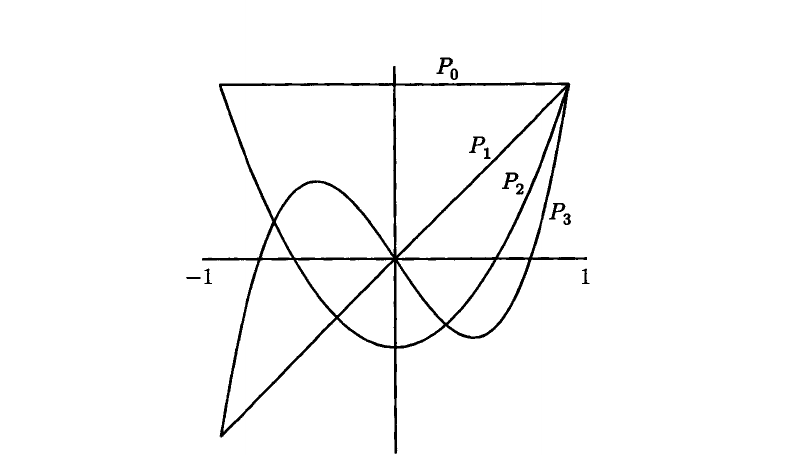
\includegraphics[width=0.68\linewidth]{../assets/figure-7-1.png}
    \caption{前四个 Legendre 多项式（式 (7.11)）.除去比例因子后，它们可以看作区间 $[-1,1]$ 上矩阵 $[1,x,x^2,x^3]$ 的约化 QR 分解中 $\widehat Q$ 的列.}
    \label{fig:legendre}
\end{figure}

Legendre 多项式构成多项式空间的一组正交基，因此也常用于谱方法.对应的正交投影为
\begin{equation}
    f(\mathord\cdot)\longmapsto
    \sum_{j=0}^{n-1}q_j(\mathord\cdot)
    \int_{-1}^{1}\overline{q_j(x)}f(x)\,dx.
    \tag{7.12}
\end{equation}

\section*{用 QR 分解求解 $Ax=b$}

最后暂时回到离散的有限矩阵.设 $A\in\C^{m\times m}$ 非奇异，并且 $A=QR$.若要解
\[
    Ax=b,
\]
左乘 $Q^*$，利用 $Q^*Q=I$ 可得
\begin{equation}
    Rx=Q^*b.
    \tag{7.13}
\end{equation}
因此可以按以下三步计算：
\begin{enumerate}[label=\arabic*.]
    \item 计算 $A=QR$.
    \item 计算 $y=Q^*b$.
    \item 回代求解上三角方程 $Rx=y$.
\end{enumerate}
这是一个很好的数值方法.第 16 讲将证明其性质.不过在实际计算中，高斯消元仍然更常用，因为它大约只需要一半的浮点运算.

\section*{习题}

\begin{enumerate}[label=\textbf{7.\arabic*}]
    \item 对习题 6.4 中的矩阵 $A$ 和 $B$，分别求出约化 QR 分解 $A=\widehat Q\widehat R$ 与完整 QR 分解 $A=QR$，并对 $B$ 做同样的计算.

    \item 假设矩阵 $A$ 的第 $1,3,5,7,\ldots$ 列与第 $2,4,6,8,\ldots$ 列彼此正交.在约化 QR 分解 $A=\widehat Q\widehat R$ 中，$\widehat R$ 具有什么特殊结构？

    \item 设 $A$ 是 $m\times m$ 矩阵，$a_j$ 是它的第 $j$ 列.证明 Hadamard 不等式
    \[
        |\det A|\le\prod_{j=1}^{m}\|a_j\|_2,
    \]
    并给出它关于平行多面体体积的几何解释.

    \item 设 $x^{(1)},y^{(1)},x^{(2)},y^{(2)}\in\R^3$ 都是非零向量，且 $x^{(1)},y^{(1)}$ 线性无关，$x^{(2)},y^{(2)}$ 也线性无关.令
    \[
        P^{(1)}=\langle x^{(1)},y^{(1)}\rangle,\qquad
        P^{(2)}=\langle x^{(2)},y^{(2)}\rangle.
    \]
    通过把问题化为三个 $3\times2$ 矩阵的 QR 分解，求出平面 $P=P^{(1)}\cap P^{(2)}$ 中的一个非零向量 $v\in\R^3$.

    \item 设 $A$ 是 $m\times n$ 矩阵（$m\ge n$），且 $A=\widehat Q\widehat R$ 是约化 QR 分解.
    \begin{enumerate}[label=(\alph*)]
        \item 证明 $A$ 的秩为 $n$ 当且仅当 $\widehat R$ 的所有对角元都非零.
        \item 如果 $\widehat R$ 有 $k$ 个非零对角元，其中 $0\le k<n$，这对 $\rank(A)$ 有什么精确含义？它给出的是相等、下界还是上界？请给出精确答案与证明.
    \end{enumerate}
\end{enumerate}

\end{document}
